\documentclass{ximera}

\newcommand{\RR}{\mathbb R}
\renewcommand{\d}{\,d}
\newcommand{\dd}[2][]{\frac{d #1}{d #2}}
\renewcommand{\l}{\ell}
\newcommand{\ddx}{\frac{d}{dx}}
\newcommand{\dfn}{\textbf}
\newcommand{\eval}[1]{\bigg[ #1 \bigg]}


\author{Bart Snapp \and Jim Talamo}

\outcome{Compute the length of a parametric curve.}

\begin{document}

%Bart, I am too busy to alter this, other than by adding the p(3) part.  In the future, I will return and write a related exercise, but I want my students to see this.  If you want this only to appear on your sample exam, please comment it out of the exercise list
\begin{exercise}
Consider the graph below of the vector-valued
function $\vec{p}(s)$. Additionally, suppose that $\vec{p}$ is
\textbf{parameterized by arc length}.
\begin{image}[4in]
    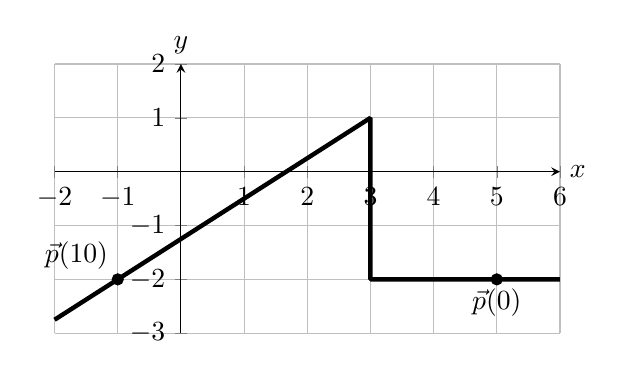
\begin{tikzpicture}
      \begin{axis}%
        [
	  xmin=-2,xmax=6,
          ymin=-3,ymax=2,
          xlabel=$x$,ylabel=$y$,
          axis lines=center,
          every axis y label/.style={at=(current axis.above origin),anchor=south},
          every axis x label/.style={at=(current axis.right of origin),anchor=west},
          clip=false,
	  grid =major,
          width=8cm,
          height=5cm,
          xtick={-2,-1,...,6},
          ytick={-3,-2,...,2},
	]
        \addplot[line join =bevel,black,ultra thick] coordinates{
          (-2,-2.75) (3,1) (3,-2) (6,-2)
        };
        \addplot[color=black,fill=black,only marks,mark=*] coordinates{(5,-2)};  %% closed hole
        \addplot[color=black,fill=black,only marks,mark=*] coordinates{(-1,-2)};  %% closed hole
        \node[black,below] at (axis cs: 5,-2) {$\vec{p}(0)$};
        \node[black,above left] at (axis cs: -1,-2) {$\vec{p}(10)$};
      \end{axis}
    \end{tikzpicture}
\end{image}

\begin{exercise}

  Compute: $\int_0^{10} \vec{p}'(s)\dotp\vec{p}'(s)\d s$
    \[
    \int_0^{10} \vec{p}'(s)\dotp\vec{p}'(s)\d s =\answer{10}
    \]
    
    \begin{hint}
    Since the curve uses arclength as a parameter, we must have that $\left|\vec{p}'(s)\right| = \answer{1}$.  How is the quantity $\vec{p}'(s)\dotp\vec{p}'(s)$ related to $\left|\vec{p}'(s)\right|$?
    
    \end{hint}
\end{exercise}
%%%%%%%%%%%%%%%%%%%%%%%%%%%%%%%%%%%%%%%%%%%%%%
\begin{exercise}
  Compute: $\vec{p}(3)$

  \[
  \vec{p}(3) = \vector{\answer{3},\answer{-1}}
  \]

\begin{hint}
Since we are given that the curve uses arclength as a parameter, $\vec{p}(3)$ can be found from the $x$ and $y$ coordinates after we travel $3$ units along the curve.  After traveling $2$ units, we arrive at $(3,-2)$, and traveling $1$ more unit brings us to $(3,-1)$.
\end{hint}
\end{exercise}
%%%%%%%%%%%%%%%%%%%%%%%%%%%%%%%%%%%%%%%%%%%%%%
\begin{exercise}
  Compute: $\vec{p}(7.5)$

  \[
  \vec{p}(7.5) = \vector{\answer{1},\answer{-.5}}
  \]

\end{exercise}
%%%%%%%%%%%%%%%%%%%%%%%%%%%%%%%%%%%%%%%%%%%%%%
\begin{exercise}
  Compute $\eval{\dd{s} \left(\vec{p}(s)\dotp\vec{p}(s)\right)}_{s=0}$

    \[
    \eval{\dd{s} \left(\vec{p}(s)\dotp\vec{p}(s)\right)}_{s=0} = \answer{-10}
    \]

 \begin{hint} 
 Using the formula for differentiating a dot product, 
 
 \[
 \dd{s} \left(\vec{p}(s)\dotp\vec{p}(s)\right) = \vec{p}'(s)\dotp\vec{p}(s) + \vec{p}(s)\dotp\vec{p}'(s) = 2 \left(\vec{p}'(s)\dotp\vec{p}(s)\right).
 \]
 
 For $0 \leq s \leq 2$, note that the curve is a horizontal line, and a tangent vector with \emph{unit} speed in the direction of the curve is $\vector{\answer{-1},\answer{0}}$, so $\vec{p}'(0) = \vector{\answer{-1},\answer{0}}$.
 
 Also, $\vec{p}(0) = \vector{\answer{5},\answer{-2}}$, so 
 
 \[
    \eval{\dd{s} \left(\vec{p}(s)\dotp\vec{p}(s)\right)}_{s=0} = 2 \left(\vec{p}'(0)\dotp\vec{p}(0)\right).
 \]
 
 
  \end{hint}
 
\end{exercise}


\end{exercise}
\end{document}
